% !TEX root = ./main.tex
\chapter{Bridge WebGL e Integrazioni Browser}
\label{app:webgl-bridge}

Nel percorso WebGL il frontend passa dal browser, ma alcune funzioni cruciali non possono essere lasciate a Unity da sola: permessi microfono, overlay DOM di Avaturn, file picker e sincronizzazione del filesystem virtuale dipendono dal contesto JavaScript della pagina. I file \texttt{.jslib} sono il punto di raccordo con questa parte del sistema.

\section{Bridge WebGL per audio e avatar}
\paragraph{\normalfont\texttt{AudioCapture.jslib}.}
Il bridge audio si occupa di tre passaggi:
\begin{itemize}
\item richiedere il permesso microfono;
\item registrare il flusso con \texttt{MediaRecorder}\footnote{\texttt{MediaRecorder} è l'API browser usata per catturare in forma registrabile un flusso audio o video già aperto.};
\item convertire il risultato in WAV PCM per il frontend.
\end{itemize}

Il lato JavaScript usa \texttt{decodeAudioData}, costruisce manualmente l'header WAV e restituisce a Unity un puntatore al buffer in memoria Emscripten\footnote{Emscripten è la toolchain che espone al modulo WebAssembly una memoria lineare condivisa con il lato JavaScript.}. Il lato C\# copia poi subito i byte con \texttt{Marshal.Copy}. È un doppio passaggio un po' grezzo, ma nel runtime WebGL si è rivelato il più stabile.

\par\begingroup
\scriptsize
\setlength{\LTleft}{0pt}
\setlength{\LTright}{0pt}
\captionsetup{type=table}
\captionof{table}{Entry point principali del bridge audio WebGL.}
\label{tab:appendix-webgl-audio-entrypoints}
\begin{longtable}{|>{\raggedright\arraybackslash}p{0.38\textwidth}|>{\raggedright\arraybackslash}p{\dimexpr0.62\textwidth-4\tabcolsep-3\arrayrulewidth\relax}|}
\hline
\textbf{Entry point} & \textbf{Funzione} \\
\hline
\endfirsthead
\hline
\textbf{Entry point} & \textbf{Funzione} \\
\hline
\endhead
\path{WebGLAudio_RequestPermission} & Chiede il permesso microfono una sola volta e notifica il risultato al client. \\
\hline
\path{WebGLAudio_StartRecording} & Avvia \texttt{MediaRecorder} sullo stream già autorizzato. \\
\hline
\path{WebGLAudio_StopRecording} & Ferma la registrazione, ricostruisce il WAV e consegna puntatore + lunghezza al callback C\#. \\
\hline
\path{WebGLAudio_CaptureFixedDuration} & Variante usata quando la durata è guidata dal flusso UI e non dal rilascio del PTT. \\
\hline
\end{longtable}
\par\endgroup

Un modo semplice di leggerlo è questo:

\begin{lstlisting}[basicstyle=\ttfamily\small,breaklines=true]
permesso microfono -> MediaRecorder
  -> blob browser
  -> decodeAudioData
  -> conversione WAV PCM
  -> _malloc in heap Emscripten
  -> callback C# con (puntatore, lunghezza)
  -> Marshal.Copy e rilascio del buffer
\end{lstlisting}

Il passaggio dati conta soprattutto perché evita due scorciatoie fragili: lasciare al browser un formato audio non controllato dal resto della pipeline, oppure demandare al backend una riconversione che il client può già gestire. In SOULFRAME il bridge audio non serve quindi solo a ``far parlare il microfono''; serve a far entrare nel sistema un WAV già compatibile con il resto del turno.

\begin{lstlisting}[style=sfcode,language={[Sharp]C},caption={Riduzione del lato C\#: il buffer viene copiato subito e poi trattato come WAV gestito.}]
[AOT.MonoPInvokeCallback(typeof(AudioDataCallback))]
private static void OnAudioReady(System.IntPtr ptr, int length)
{
    var managedBytes = new byte[length];
    Marshal.Copy(ptr, managedBytes, 0, length);
    recorder.DeliverWav(managedBytes);
}
\end{lstlisting}

\paragraph{\normalfont\texttt{AvaturnBridge.jslib}.}
Il bridge Avaturn crea un overlay DOM a schermo intero, inizializza l'SDK e inoltra l'evento di export a Unity tramite \texttt{SendMessage}\footnote{\texttt{SendMessage} è il meccanismo con cui uno script browser richiama un metodo pubblico di un oggetto Unity già presente in scena.}. Il pacchetto JSON che rientra in Unity è simile al seguente:

\begin{lstlisting}[language=json,caption={Payload di export inoltrato dal bridge Avaturn al client Unity.}]
{
  "url": "https://api.avaturn.me/avatars/exports/.../model",
  "urlType": "httpURL",
  "bodyId": "body_1",
  "gender": "male",
  "avatarId": "019c8296-1a77-75b1-9d4b-c36ff20d1a4c"
}
\end{lstlisting}

Lo stesso bridge gestisce anche apertura, chiusura e ritorno del focus al canvas Unity. È un dettaglio poco appariscente, ma importante per evitare che il browser resti ``agganciato'' all'overlay dopo la chiusura dell'editor avatar.

\begin{lstlisting}[style=sfcode,language={[Sharp]C},caption={Estratto adattato del callback che rientra in Unity dopo l'export Avaturn.}]
public void OnAvatarJsonReceived(string json)
{
    var jsonData = JsonUtility.FromJson<AvatarJsonData>(json);
    if (jsonData != null && jsonData.status == "closed")
        SetWebOverlayOpen(false);

    avatarManager.OnAvatarJsonReceived(json);
}
\end{lstlisting}

Nel file il flusso reale è questo:

\begin{lstlisting}[basicstyle=\ttfamily\small,breaklines=true]
OpenAvaturnIframe
  -> crea overlay e iframe
  -> prova a caricare l'SDK Avaturn
  -> intercetta export / cancel / error
  -> serializza il payload
-> prova SendMessage su piu varianti di istanza Unity
  -> chiude overlay e rifocalizza il canvas
\end{lstlisting}

Il tentativo su più varianti di \texttt{SendMessage} serve perché i template WebGL non espongono sempre l'istanza Unity nello stesso modo; senza questa cautela il bridge diventerebbe fragile proprio nelle build che dovrebbero essere più portabili.

Anche qui il punto non è cosmetico. Overlay, callback e refocus non servono soltanto a chiudere bene l'editor avatar: servono a evitare che DOM e canvas Unity si contendano tastiera, click e stato della pagina proprio durante un passaggio delicato dell'onboarding.

\section{Integrazioni browser e filesystem virtuale}
\paragraph{\normalfont\texttt{WebGLFilePicker.jslib} e file picker browser.}
Il file picker WebGL serve soprattutto a \texttt{SetupMemory}. Il plugin apre il selettore di file del browser, converte il contenuto in base64 e lo rimanda al client come piccolo JSON. In questo modo il frontend può trattare in modo abbastanza uniforme selezione documento e selezione immagine, pur restando dentro i vincoli della pagina web.

\begin{lstlisting}[language=json,caption={Payload tipico del file picker WebGL verso Unity.}]
{
  "name": "schema.pdf",
  "type": "application/pdf",
  "size": 84213,
  "data": "JVBERi0xLjcKJc..."
}
\end{lstlisting}

Questo schema separa il gesto di selezione dal modo in cui il file verrà poi usato. Il client riceve un oggetto abbastanza regolare da poterlo inoltrare al backend come documento da ingestire o come immagine da descrivere, senza dover costruire due pipeline completamente diverse solo perché il browser consegna dati in modo scomodo.

\paragraph{\normalfont\texttt{fs.jslib} e sincronizzazione del filesystem virtuale.}
Il progetto include anche \texttt{fs.jslib}, che espone helper come \texttt{EnsureDynCallV}, \texttt{JS\_FileSystem\_Sync} e \texttt{JS\_FileSystem\_SyncFromDiskAndNotify}. Nel flusso attuale questa parte non è la fonte canonica del catalogo avatar: il manager usa comunque il backend come punto di verità. Il bridge rimane però utile come supporto di compatibilità per alcuni stati del browser.

Anche qui il dettaglio utile non è l'intera API, ma i messaggi che il bridge rimanda a Unity: \texttt{OK}, \texttt{ERR:no\_fs} oppure \texttt{ERR:<messaggio>}. Questa codifica minima basta a distinguere un sync riuscito, un browser privo di \texttt{FS.syncfs} e un errore runtime più specifico, senza introdurre un protocollo più pesante.

Nel progetto è stato facile fraintendere un punto: esiste una UI touch abbastanza articolata, con gesture, swipe e pulsanti PTT dedicati, ma questo non significa che esista già un client mobile nativo separato. Oggi il touch è un adattamento della stessa esperienza WebGL, non un'app autonoma con ciclo di vita distinto.

La Figura~\ref{fig:appendix-avaturn-overlay} mostra il caso più rappresentativo di questa integrazione browser-side: il configuratore Avaturn viene aperto come overlay web sopra il flusso di SOULFRAME e il client Unity riprende il controllo solo quando il browser restituisce l'avatar selezionato tramite callback.

\begin{figure}[H]
    \centering
    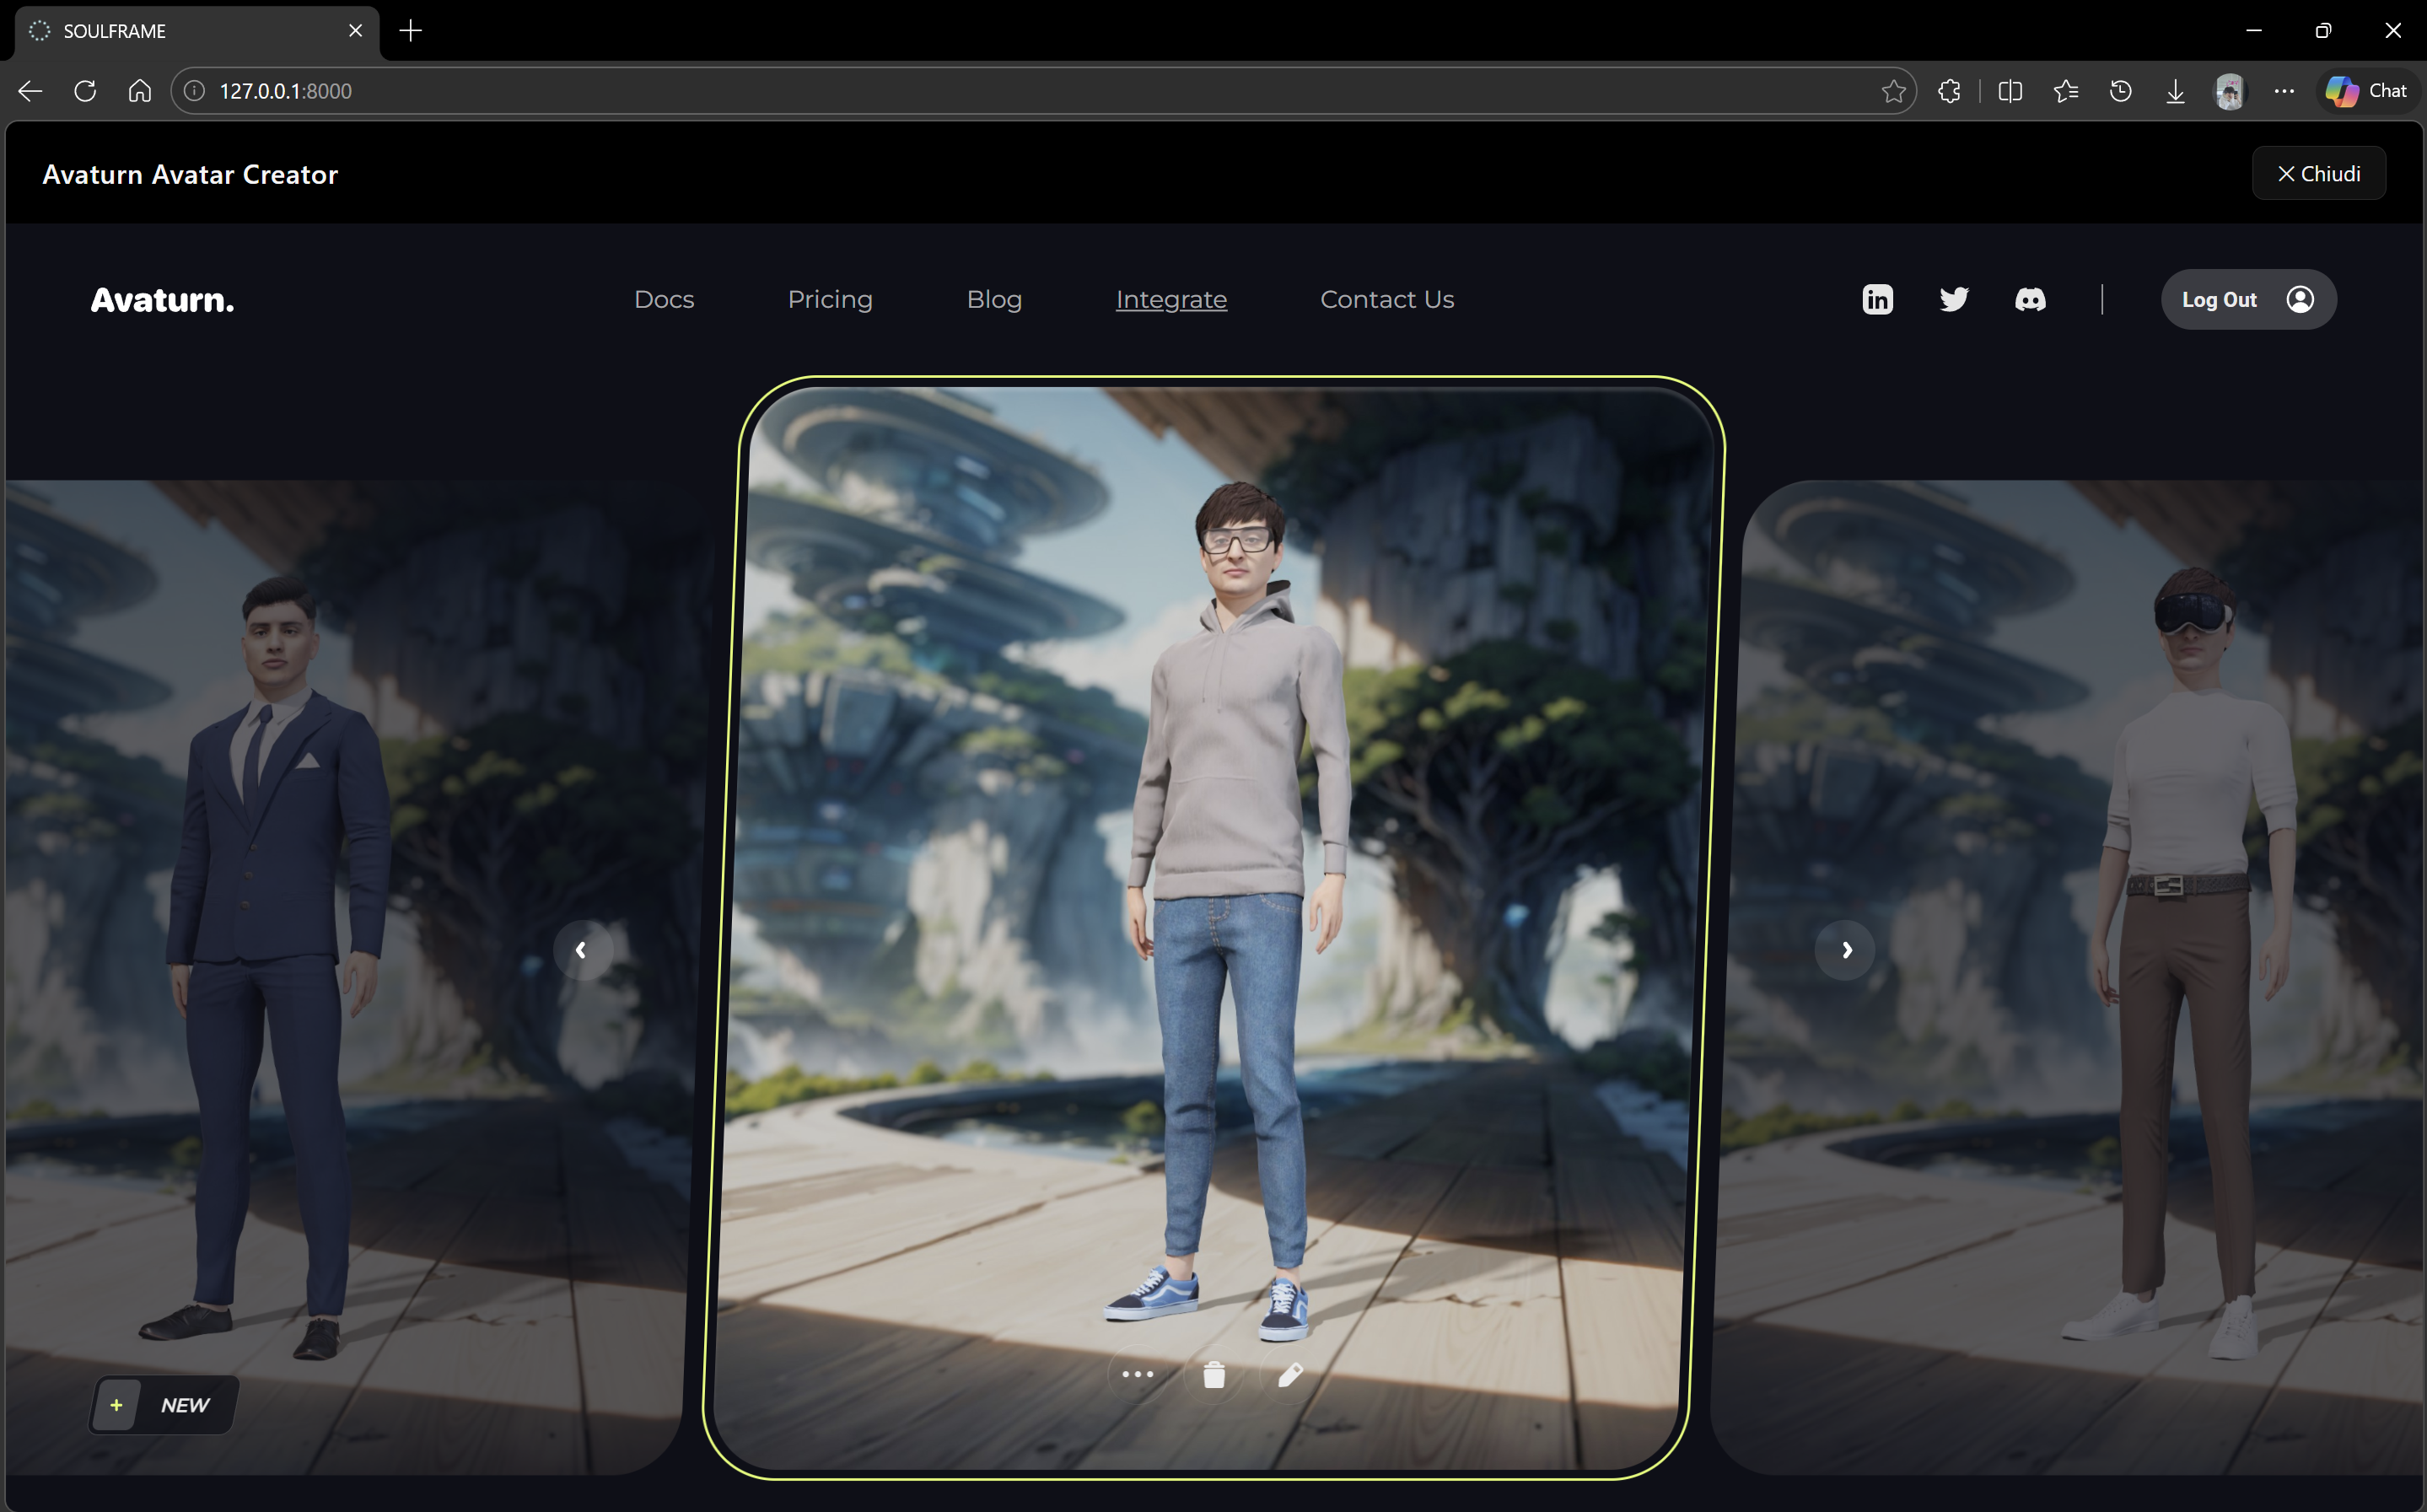
\includegraphics[width=0.96\textwidth]{Risorse/ui_avaturn_overlay_webgl.png}
    \caption{Overlay del configuratore Avaturn aperto nel flusso WebGL di SOULFRAME. Il client Unity resta sospeso finché il browser non restituisce l'avatar selezionato tramite callback.}
    \label{fig:appendix-avaturn-overlay}
\end{figure}
